% Standalone IEEE-style manuscript. Compile twice with pdfLaTeX.
% Scope: repository revision 266499b, inspected October 4, 2026.
% Replace the author block and complete declarations before submission.
% No clinical cohort, trained model evaluation, or patient outcome study is claimed.
\documentclass[conference]{IEEEtran}
\usepackage[T1]{fontenc}
\usepackage[utf8]{inputenc}
\usepackage{cite}
\usepackage{amsmath,amssymb}
\usepackage{booktabs,array,tabularx}
\usepackage{xurl}
\usepackage[hidelinks]{hyperref}
\usepackage{listings}
\usepackage{tikz}
\usetikzlibrary{arrows.meta,positioning,fit,backgrounds}
\lstset{basicstyle=\ttfamily\scriptsize,breaklines=true,columns=fullflexible,keepspaces=true,showstringspaces=false}
\newcolumntype{Y}{>{\raggedright\arraybackslash}X}
\newcommand{\system}{PulseGraph AI}
\newcommand{\code}[1]{\texttt{\detokenize{#1}}}

\title{PulseGraph AI: Design and Software Verification of a Graph-Orchestrated Clinical Decision-Support Prototype}
\author{\IEEEauthorblockN{Author Name(s)}
\IEEEauthorblockA{Department and Institution\\City, Country\\Email Address}}

\begin{document}
\maketitle

\begin{abstract}
Clinical decision-support workflows must manage incomplete information, contextual symptom descriptions, assessment applicability, and clinician oversight. A system that converts every recognized symptom into a disease-specific questionnaire can create unnecessary requests and conceal gaps in its clinical coverage. This paper presents PulseGraph AI, a graph-orchestrated research prototype that separates intake, presentation extraction, urgency screening, calculator routing, data acquisition, and clinician review. The implementation combines typed clinical state, deterministic symptom-context extraction with source spans, a limited versioned observation screen, clinician-confirmed applicability for three existing calculators, and resumable requests for missing information. Presentations outside the implemented assessment coverage terminate with an explicit clinician-assessment handoff. The architecture also contains imaging, diagnostic, evidence, pharmacology, and symbolic-rule nodes; several of these remain demonstration components rather than validated AI services. A focused evaluation of the current implementation executed 121 automated regression tests, all of which passed. These tests establish specified software behaviors in an isolated environment, not clinical effectiveness. The paper contributes an inspectable workflow design, an explicit representation of incomplete and unsupported assessments, a reproducible software-verification account, and a staged plan for clinical evaluation. General diagnostic capability, optional imaging, model-based retrieval, and real-world clinical benefit remain unestablished.
\end{abstract}

\begin{IEEEkeywords}
clinical decision support, workflow orchestration, clinical triage, contextual extraction, human-in-the-loop systems, software verification
\end{IEEEkeywords}

\section{Introduction}
Clinical decision-support systems (CDSSs) combine patient information and clinical knowledge to assist decisions at the point of care. Their value depends on more than a correct calculation: input quality, workflow fit, presentation of uncertainty, and user interaction influence whether the output is useful. Sutton \emph{et al.} describe both the benefits and implementation risks of CDSSs, including challenges associated with adoption and maintenance \cite{sutton}. Topol situates medical AI within a broader relationship between computational capabilities and human clinical work \cite{topol}. These perspectives motivate systems that make their scope and decision process visible to the clinician.

Recent language-model research has demonstrated substantial medical knowledge on question-answering tasks \cite{singhal}. Such evidence does not by itself demonstrate that a complete clinical workflow can reliably collect information, detect contradictory statements, determine which assessment is appropriate, or recover from missing data. An application can expose an apparently fluent clinical interface while relying on a narrow set of assumptions underneath. Conversely, a useful early research contribution can consist of explicit workflow controls without claiming a new diagnostic model.

\system{} addresses this engineering problem through a stateful graph of specialized processing nodes. The current implementation has progressed from symptom-triggered cardiopulmonary calculators toward broader presentation grouping with explicit assessment boundaries. A complaint outside the implemented calculators can be represented and handed to a clinician instead of being forced into a chest-disease workflow. This is broader \emph{routing coverage}, not comprehensive disease coverage.

This paper reports the repository at revision \code{266499b}, inspected on October 4, 2026, after the fourth phase of the triage roadmap. Its contributions are: (1) a typed, resumable clinical-workflow architecture; (2) source-linked symptom interpretation and explicit applicability decisions; (3) operational handling of unknown, unavailable, and unsupported information; and (4) a software evaluation with a clearly bounded interpretation. The research questions are whether the implementation preserves intake across pauses, prevents automatic calculator activation without applicability decisions, and routes incomplete or unsupported cases to an explicit handoff. The paper does not test whether the system improves diagnosis, treatment, or patient outcomes.

\section{Problem Statement and Design Objectives}
\subsection{The Workflow Problem}
Consider a patient whose intake already includes a chief complaint and presenting symptoms. Requiring the same information immediately after patient selection introduces duplicate entry and creates an opportunity for disagreement between records. A second problem occurs when a phrase such as breathlessness automatically activates every associated calculator. Symptoms can suggest candidate assessments, but they do not establish that the patient belongs to each calculator's intended clinical context.

A third problem concerns missingness. An absent answer, an explicitly negative answer, a historical finding, and a measurement that cannot be obtained are different observations. Treating any of them as a normal value can produce an apparently complete but unsupported assessment. Finally, a completed calculator for one complaint can obscure a second complaint for which no implemented pathway exists.

The design problem is therefore to organize a clinical support workflow that preserves these distinctions while allowing supported work to proceed. In this paper, ``triage'' names the application's intake, urgency, and assessment-routing functions. It does not imply validation as an emergency-department triage scale or autonomous disposition system.

\subsection{Requirements}
The prototype is designed around six requirements:
\begin{enumerate}
\item Reuse persisted intake and validated observations across session execution and data-request resolution.
\item Preserve contextual symptom assertions and their originating text.
\item Evaluate the limited urgency screen before routine questionnaires and reassess when relevant inputs change.
\item Separate a candidate assessment from clinician-confirmed applicability.
\item Represent incomplete and unsupported work without inventing measurements or implying low risk.
\item Require explicit clinician interaction at designated checkpoints and retain a reviewable audit history.
\end{enumerate}
These are design objectives with selected regression checks, not formally proven guarantees for every possible input or execution schedule.

\section{Literature Review}
\subsection{Contextual Clinical Text Processing}
Clinical text cannot be interpreted reliably using symptom presence alone. NegEx introduced a practical rule-based approach to identifying negated findings in clinical reports \cite{negex}. ConText extended contextual analysis to dimensions such as experiencer and temporal status \cite{context}. These studies motivate the separation of a symptom mention from an assertion about the current patient.

PulseGraph uses a bounded deterministic English extractor rather than a reproduction of either algorithm. It retains categories for present, absent, historical, uncertain, other-person, and conflicting assertions. Its relationship to this literature is conceptual: context changes the meaning of a detected term. No benchmark comparison with NegEx, ConText, or a clinical language model has been conducted. Exact source spans make an extraction inspectable but do not establish that its interpretation is correct.

\subsection{Clinical Prediction Rules and Applicability}
The HEART score was introduced for chest-pain assessment in the emergency setting \cite{heart}. CURB-65 arose from a study of community-acquired pneumonia severity on presentation to hospital \cite{curb}. Wells \emph{et al.} evaluated a clinical model within a diagnostic strategy for patients with suspected pulmonary embolism \cite{wells}. These studies concern defined patient populations and clinical tasks; their existence does not validate arbitrary use based on a symptom keyword.

PulseGraph incorporates implementations of these three calculators, but this paper evaluates the surrounding workflow rather than deriving or externally validating the scores. The router asks for clinician confirmation before calculator-specific questions. Existing numerical formulas and interpretation strings were retained during the routing phase. Accordingly, original validation results and risk estimates from the literature must not be attributed to PulseGraph's implementation or user population.

\subsection{Retrieval and Agent-Oriented Systems}
Retrieval-augmented generation combines generation with access to an external information source \cite{rag}. ReAct investigates interleaving reasoning and actions in language-model systems \cite{react}. These approaches motivate separating knowledge access, tool execution, and response construction. They do not imply that every application with multiple named nodes implements autonomous model-driven agents.

In PulseGraph, an agent is currently a specialized state-processing function. Graph orchestration provides explicit routing and interruption points; it does not establish cooperative intelligence or emergent clinical reasoning. The evidence node presently selects fixed citation records, so it is not an evaluated retrieval-augmented generation system. The distinction between interface names and executable behavior is central to the implementation audit reported here.

\subsection{Evaluation of Clinical AI}
DECIDE-AI addresses reporting of early clinical evaluations, emphasizing the interaction between a system, its users, and its clinical environment \cite{decide}. CONSORT-AI addresses reporting for trials of AI interventions \cite{consort}. TRIPOD+AI provides reporting guidance for prediction-model studies using regression or machine learning \cite{tripod}. These publications concern different study types and stages.

The present work is a software prototype study. It has neither a live clinical investigation nor a prediction-model development dataset, and it does not claim compliance with those checklists as a substitute for such studies. They instead inform the future evaluation plan: evaluate workflow and human factors before claiming clinical utility, and report any subsequently trained prediction models and comparative trials using guidance appropriate to their designs.

\subsection{Research Position}
The contribution is an integration and verification account, not a claim that clinical calculators, contextual extraction, or graph execution are individually novel. PulseGraph makes the boundary between supported calculation and incomplete assessment an explicit workflow outcome. Its suitability for publication rests on transparent implementation reporting and a reproducible evaluation, while comparative novelty and clinical benefit remain research questions.

\subsection{Human Factors and Automation Bias}
Goddard, Roudsari, and Wyatt review automation bias and the factors that influence reliance on decision aids \cite{automation}. Their work motivates an important distinction for PulseGraph: requiring a click is not equivalent to obtaining an independent clinical judgment. A user may acknowledge an alert simply to continue a task. Thus, acknowledgement is a workflow event whose clinical meaning depends on interface design, workload, training, and the response process. This manuscript makes no claim that the existing acknowledgement mechanism eliminates automation bias.

For the proposed usability evaluation, the relevant question is whether clinicians can accurately explain why a pathway was selected, which information remains unavailable, and what the system has not assessed. These are application-specific hypotheses. Testing them requires observing interactions and errors, not merely counting successful API responses. A clinician can complete a software task while misunderstanding the scope of the output; that distinction should be part of the outcome definition.

\subsection{Bias, Subgroups, and Distribution Shift}
Obermeyer \emph{et al.} show how a healthcare algorithm can exhibit racial bias when its prediction target is an imperfect proxy for the intended health construct \cite{obermeyer}. For PulseGraph, the methodological implication is to specify the decision being supported and the meaning of the reference label before developing predictive components. An observed treatment, test order, or resource-use variable should not automatically become a label for what should have happened. This is a proposed evaluation principle, not evidence that the current router is equitable.

Oakden-Rayner \emph{et al.} discuss hidden stratification, in which broad labels conceal clinically meaningful subsets with different model performance \cite{hidden}. A single aggregate result for ``respiratory complaints'' could similarly obscure failures on unusual wording, mixed presentations, or unavailable observations. Finlayson \emph{et al.} describe dataset shift and its implications for deployed medical AI \cite{shift}. These concerns motivate separate checks of language, population, and workflow changes when transferring a future PulseGraph model between settings. The deterministic components also depend on input conventions, although their failure mechanisms differ from those of learned models.

The proposed analysis should therefore distinguish observed subgroup differences from their possible causes. Small subgroup samples may produce unstable estimates, and a nominally similar average metric can hide unequal handoff burden. Recording denominators, uncertainty intervals, missingness rates, and assessment coverage would make those limitations visible. None of these subgroup analyses has yet been performed.

\subsection{Calibration and Evidence Quality}
Guo \emph{et al.} study calibration of neural-network confidence estimates \cite{calibration}. Their results concern learned predictors; they do not make a fixed demonstration confidence value meaningful. If PulseGraph later displays probabilities from an imaging or diagnostic model, those values should be evaluated against a defined outcome and population. Routing statuses such as incomplete or unsupported should remain distinct from numeric confidence, since they describe what work was performed rather than an estimated event probability.

Nagendran \emph{et al.} examine design, reporting, and claims in studies comparing AI with clinicians \cite{nagendran}. Roberts \emph{et al.} identify methodological problems in machine-learning studies of COVID-19 imaging \cite{roberts}. These reviews support caution in moving from retrospective performance to clinical claims. For this project, a technically successful image classifier would still leave unanswered questions about image acquisition, clinical indication, downstream actions, and clinician response. Evaluation must include the workflow surrounding the classifier rather than treating its benchmark score as a system-level result.

Wiens \emph{et al.} outline a roadmap for responsible healthcare machine learning \cite{wiens}. PulseGraph's proposed development stages adopt the general principle that problem formulation, evaluation, and deployment responsibilities must be considered together. The manuscript does not claim to have executed that roadmap. Its present role is to identify what the prototype can demonstrate and what evidence would be necessary for a stronger claim.

\subsection{Clinical Data Resources and Study Fit}
MIMIC-IV is an electronic-health-record research resource described by Johnson \emph{et al.} \cite{mimic}. It is a possible source for future retrospective research under its access requirements, not a dataset used in this paper. Availability of an EHR dataset does not ensure that it contains the exact intake language, clinician applicability decisions, or unavailable-data reasons needed to evaluate PulseGraph. Such labels may require a separately designed annotation study.

Dataset selection should follow the research question. Testing extraction requires source text and contextual annotations; testing calculator applicability requires adjudication of clinical context; testing recovery requires controlled execution failures; and testing clinician comprehension requires human participants. No single dataset can substitute for all four. This division also prevents a future study from presenting a large number of retrospective records as evidence for interface behavior that those records do not observe.

\section{Methodology}
\subsection{Study Design and Evidence Sources}
The study combines a source-code inspection with execution of a focused automated regression suite. Inspection covered clinical state schemas, presentation extraction, urgency rules, routing, calculator calls, graph transitions, request validation, service persistence, and the user-interface components exposing these results. It also examined downstream nodes to distinguish implemented services from demonstrations.

The literature review is a targeted narrative review, not a systematic review. Searches selected original calculator studies, foundational contextual-extraction and retrieval papers, clinical-AI reporting statements, and official technical or guideline documentation directly relevant to implementation decisions. Bibliographic details were checked against publisher, PubMed, conference, author-preprint, or issuing-organization records. No exhaustive search strategy, screening flow, or formal risk-of-bias assessment is claimed.

The regression suite uses developer-authored synthetic fixtures. API tests in the selected intake/routing fixtures use SQLite and in-memory graph checkpoints, with a test clinician supplied through dependency overrides. No patient cohort was collected or analyzed for this paper. Test counts are counts of software cases, including parameterized cases, rather than numbers of patients or independent clinical observations.

\subsection{State Representation}
Let the workflow state at step $t$ be
\begin{equation}
S_t=(D,V,N,P,U,R,Q,O,A,C)_t,
\end{equation}
where $D$ contains demographics and recorded history, $V$ contains observations, $N$ contains source notes, $P$ is the structured presentation, $U$ is the urgency assessment, $R$ contains routing and score information, $Q$ contains data requests, $O$ contains downstream outputs, $A$ is the audit history, and $C$ contains clinician/session control information. This tuple is an explanatory abstraction of the implementation rather than a distinct serialized data structure.

Each graph node produces a partial state update:
\begin{equation}
S_{t+1}=S_t\oplus f_i(S_t),
\end{equation}
where $f_i$ is a node function and $\oplus$ applies field-specific update behavior. Clinical schemas use Pydantic validation. Notes and audit events can accumulate, while the current triage score set replaces prior triage-pass scores to avoid retaining results for paths that no longer apply. Persistent session/results storage and graph checkpoints have separate roles: the former exposes application records and the latter preserves resumable execution state.

\subsection{Intake and Source Preservation}
Session intake persists notes and structured observations. Execution can reuse the saved chief complaint instead of demanding duplicate symptom entry. Numeric parsing rejects malformed strings, non-finite values, and inappropriate boolean-to-number conversion. Assessment categories are validated against allowed values rather than accepted as arbitrary text.

For a source text $x$, an extracted mention records a span $(a,b)$ and quote $q$ such that
\begin{equation}
q=x[a:b].
\end{equation}
The extractor associates each supported symptom with contextual status and, where its bounded patterns permit, time course, severity, or location. Ambiguous attributes are left unknown. Conflicting positive and negative assertions prompt clarification while retaining original evidence. Unrecognized wording remains available to the clinician; it is not converted into a normal finding.

This design supports traceability within the recognized vocabulary. It does not establish complete recall: a note may contain a supported symptom alongside an unrecognized urgent complaint. Retaining raw text mitigates information loss but cannot guarantee that the routing stage recognizes every concern.

\subsection{Limited Urgency Screening}
An \code{urgency_check} node precedes triage, runs after resolved clinical data requests, and precedes clinician-requested diagnostic reevaluation. Its candidate observation thresholds draw on individual extreme-observation bands in NEWS2 \cite{news2}; explicit clinician concern is also represented, consistent with the importance assigned to concern in NICE CG50 \cite{cg50}. The implementation does not calculate a NEWS2 aggregate or implement its complete escalation protocol.

Physiological screening requires recorded age of at least 16 years and explicit non-pregnancy. Oxygen-saturation screening additionally requires confirmation that the standard scale is appropriate. Explicit clinician concern can trigger review independently of those restrictions. The assessment distinguishes urgent review, incomplete assessment, outside-scope input, and no detected trigger. None of the latter three states establishes clinical safety.

An urgent finding creates a request that requires acknowledgement by the session's authenticated clinician. A fingerprint derived from observations, context, revision information, and rule configuration associates the acknowledgement with the evaluated state. Changed inputs invalidate the previous acknowledgement. Acknowledging permits workflow continuation; it does not erase the finding or certify that treatment has occurred. Defaults remain marked as pending clinical review. The implementation does not evaluate measurement freshness, trends, or the cumulative importance of multiple moderate abnormalities.

\subsection{Presentation Groups and Calculator Selection}
The router preserves nine descriptive groups: cardiovascular, respiratory, vascular, gastrointestinal, neurological, skin, urinary, musculoskeletal/injury, and systemic. Groups are not diagnoses. Only three calculator pathways currently exist, so most groups have no corresponding automated assessment.

For each candidate pathway $j$, the clinician decision is
\begin{equation}
d_j\in\{\mathrm{applicable},\mathrm{not\ applicable},\mathrm{unknown}\}.
\end{equation}
An unanswered decision remains distinct from an explicit unknown decision. Candidate selection uses recognized current-positive symptoms. Applicability confirmation precedes calculator input collection. For example, the CURB-65 prompt asks whether an adult hospital presentation has a clinical diagnosis of community-acquired pneumonia, reflecting its clinical context in NICE NG250 \cite{nicepneumonia}. The Wells prompt asks whether pulmonary embolism is clinically suspected, as distinguished from symptom detection in NG158 \cite{nicepe}. The application does not implement those guidelines in full; in particular, its retained Wells interpretation is not a complete implementation of the NICE two-level management pathway.

Routing conservatively excludes recorded age below 18 and known pregnancy from these calculators. These are software coverage restrictions, not universal claims about each score's validated population. Missing age is requested, while unavailable age produces a handoff. Pregnancy handling differs between components: the urgency screen requires explicit non-pregnancy, whereas calculator routing excludes known pregnancy. This difference is documented rather than treated as a uniform eligibility policy.

\subsection{Targeted Questions and Unavailable Information}
Let $F_j$ be a pathway's required field set and $K_t$ the set of usable fields already recorded. For a confirmed pathway, the requested set is
\begin{equation}
M_j=F_j\setminus K_t.
\end{equation}
The implementation permits selected triage fields to carry an explicit unavailable marker. Such a marker is not inserted into numeric observations and does not become a negative boolean answer. Instead, it marks the affected assessment incomplete and prevents the same unavailable field from being requested indefinitely. Other applicable assessments may still complete.

A recognized current concern that is not covered by completed or pending supported work remains a handoff reason. The terminal status \code{REQUIRES_CLINICIAN_ASSESSMENT} distinguishes this outcome from ordinary completion. The graph stops before downstream imaging and diagnosis in such cases. This mechanism protects the supported vocabulary against silent coverage loss; it is not an open-world detector of all unsupported clinical concepts.

\section{System Architecture and Implementation}
Figure~\ref{fig:architecture} presents the application layers and the principal execution branches. Solid arrows show the current control or service relationships at an architectural level; dashed boxes denote demonstration components or planned work, as labeled. The data-request checkpoint is shared by requesting nodes, and resolution returns through urgency reassessment before the selected continuation. The figure abstracts individual API endpoints and does not imply that all database updates form a single transaction.

\begin{figure*}[t]
\centering
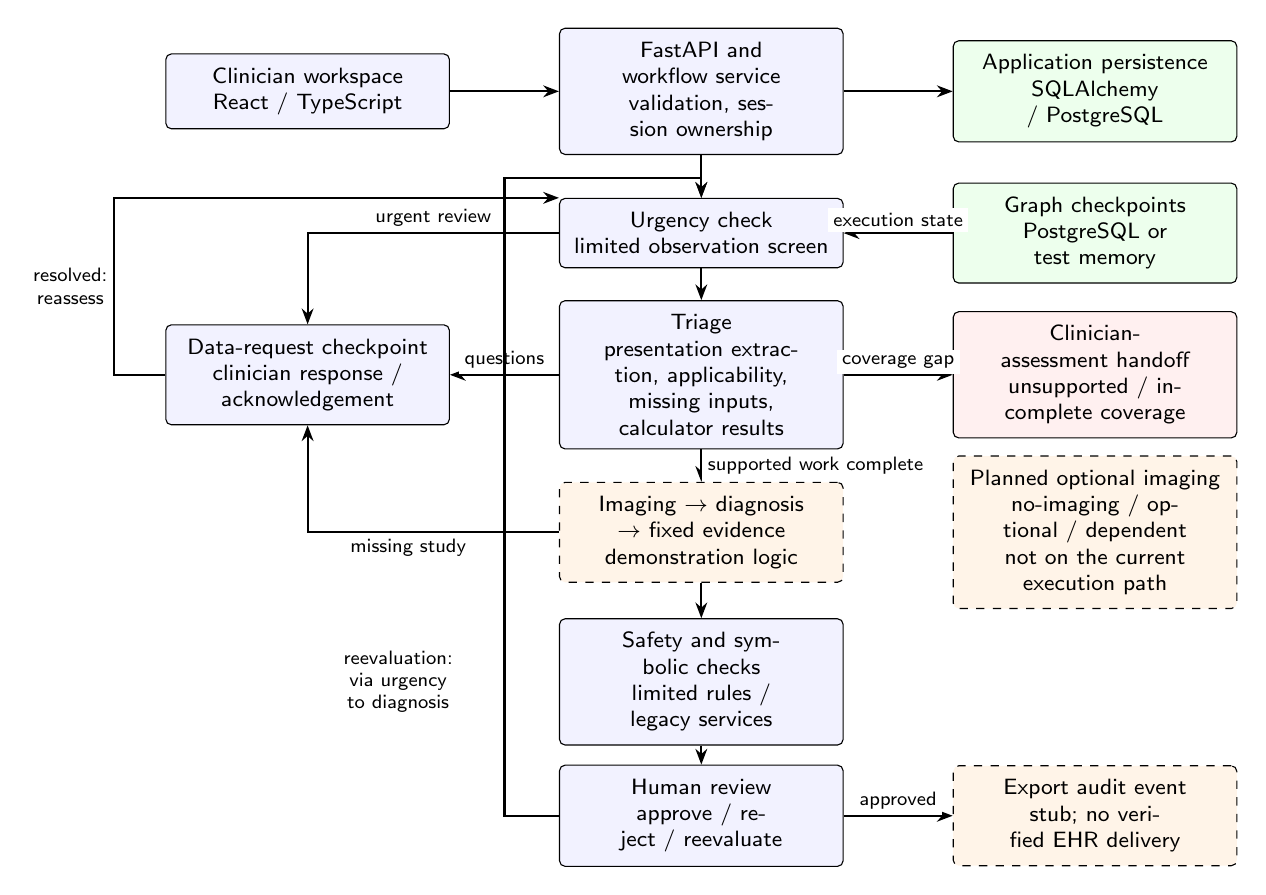
\begin{tikzpicture}[
 font=\sffamily\footnotesize,
 box/.style={draw,rounded corners=2pt,align=center,minimum height=0.85cm,text width=3.25cm,inner sep=5pt,fill=blue!5},
 demo/.style={box,dashed,fill=orange!9},
 store/.style={box,fill=green!7},
 flow/.style={-{Stealth[length=2mm]},thick},
 note/.style={font=\sffamily\scriptsize,align=center,fill=white,inner sep=2pt}
]
\node[box] (ui) at (0,0) {Clinician workspace\\React / TypeScript};
\node[box] (api) at (5,0) {FastAPI and workflow service\\validation, session ownership};
\node[store] (db) at (10,0) {Application persistence\\SQLAlchemy / PostgreSQL};
\node[box] (urgency) at (5,-1.8) {Urgency check\\limited observation screen};
\node[store] (checkpoint) at (10,-1.8) {Graph checkpoints\\PostgreSQL or test memory};
\node[box] (request) at (0,-3.6) {Data-request checkpoint\\clinician response / acknowledgement};
\node[box] (triage) at (5,-3.6) {Triage\\presentation extraction, applicability,\\missing inputs, calculator results};
\node[box,fill=red!6] (handoff) at (10,-3.6) {Clinician-assessment handoff\\unsupported / incomplete coverage};
\node[demo] (downstream) at (5,-5.6) {Imaging $\rightarrow$ diagnosis\\$\rightarrow$ fixed evidence\\demonstration logic};
\node[demo] (future) at (10,-5.6) {Planned optional imaging\\no-imaging / optional / dependent\\not on the current execution path};
\node[box] (safety) at (5,-7.5) {Safety and symbolic checks\\limited rules / legacy services};
\node[box] (review) at (5,-9.2) {Human review\\approve / reject / reevaluate};
\node[demo] (export) at (10,-9.2) {Export audit event\\stub; no verified EHR delivery};
\draw[flow] (ui) -- (api);
\draw[flow] (api) -- (db);
\draw[flow] (api) -- (urgency);
\draw[flow] (urgency) -- (triage);
\draw[flow] (checkpoint) -- node[note,above]{execution state} (urgency);
\draw[flow] (triage) -- node[note,above]{coverage gap} (handoff);
\draw[flow] (triage) -- node[note,right]{supported work complete} (downstream);
\draw[flow] (downstream) -- (safety);
\draw[flow] (safety) -- (review);
\draw[flow] (review) -- node[note,above]{approved} (export);
\draw[flow] (triage) -- node[note,above]{questions} (request);
\draw[flow] (urgency.west) -| node[note,pos=0.25,above]{urgent review} (request.north);
\draw[flow] (request.west) -- ++(-0.65,0) |- node[note,pos=0.25,left]{resolved:\\reassess} (urgency.north west);
\draw[flow] (downstream.west) -| node[note,pos=0.3,below]{missing study} (request.south);
\draw[flow] (review.west) -- (2.5,-9.2) -- (2.5,-1.1) -| (urgency.north);
\node[note,text width=2.2cm] at (1.15,-7.5) {reevaluation:\\via urgency\\to diagnosis};
\end{tikzpicture}
\caption{PulseGraph architecture at the inspected revision. The diagram separates the implemented triage controls, current downstream demonstrations, persistent state, and planned imaging extension. Other downstream nodes can also request data; their checkpoint edges are omitted for readability. Rejection ends in manual takeover, and no external emergency notification or EHR delivery is implied.}
\label{fig:architecture}
\end{figure*}
\subsection{Application Layers}
The backend uses FastAPI for endpoints, SQLAlchemy for application persistence, Alembic for migrations, and LangGraph for execution control. LangGraph supports stateful graph execution and interruption mechanisms \cite{langgraph}. PostgreSQL checkpointing is available, while in-memory checkpoints support isolated testing. Production configuration rejects a non-PostgreSQL checkpoint backend; development configuration may fall back to memory after initialization failure. This policy does not itself prove recovery correctness under process crashes or network failures.

The React/TypeScript frontend exposes intake, data requests, triage results, urgency information, and review actions. Applicability decisions have no preselected clinical answer. Eligible fields expose an unavailable option. Routing status and handoff reasons are visible, and polling terminates when manual assessment is required. A second initial run of an already-started session returns HTTP 409 rather than creating another pending questionnaire.

\begin{table*}[t]
\caption{Implementation Scope at the Inspected Revision}
\label{tab:scope}
\centering\small
\begin{tabularx}{\textwidth}{p{0.16\textwidth}YY}
\toprule
Component & Implemented behavior & Boundary of the present evidence \\
\midrule
Intake and presentation & Persisted intake; typed observations; contextual extraction; exact text spans & Bounded English patterns, without clinical-corpus accuracy estimates \\
Urgency & Versioned observation rules; explicit concern; acknowledgement and reassessment & Candidate limited screen, not NEWS2 or comprehensive emergency triage \\
Triage routing & Nine presentation groups; three calculators; applicability and handoff & Additional disease-specific pathways are not implemented \\
Imaging & Image-path acquisition and filename-dependent simulated findings & No pixel-based model inference or validated image interpretation \\
Diagnosis & Keyword and imaging-label rules producing structured differentials & No trained diagnostic model or measured diagnostic performance \\
Evidence & Fixed citation records selected from differential labels & No live document retrieval, ranking evaluation, or generated grounded answer \\
Pharmacology & Drug-name lookup code, interaction API call code, and local fallback rules & External interaction endpoint is obsolete; fallback coverage is limited \\
Symbolic checks & Explicit conditional rules producing override records & Clinical correctness and completeness are not established \\
Review and export & Review checkpoint, bounded reevaluation, export-status audit event & Export event is a stub, not verified EHR delivery \\
\bottomrule
\end{tabularx}
\end{table*}

\subsection{Execution and Review}
The principal implemented sequence is intake, urgency, triage, imaging, diagnosis, evidence, safety, symbolic checks, and human review. Conditional edges interrupt that sequence when a node requests data. Unsupported triage outcomes terminate early. A resolved request routes through urgency reassessment before resuming the appropriate processing node.

Human review permits approval, rejection/manual takeover, or a bounded reevaluation loop. Reevaluation appends clinician feedback and resumes diagnostic processing after urgency checking; it is not a complete rerun of all preceding assessments. The current maximum reevaluation count is two. This bound concerns the implemented diagnostic feedback loop and is not a general proof of termination for all data-acquisition sequences.

The following pseudocode summarizes the core triage control policy, omitting persistence and API details:
\begin{lstlisting}
load persisted intake and available observations
evaluate limited urgency screen
if unacknowledged urgent finding:
    pause for authorized clinician review
extract contextual presentation with source spans
if unresolved assertion conflict:
    request clarification; pause
identify candidate calculators and coverage gaps
if applicability decisions are unanswered:
    request applicable / not_applicable / unknown
for each confirmed, supported calculator:
    if a required input is explicitly unavailable:
        record incomplete assessment
    elif required usable inputs are missing:
        request missing inputs; pause
    else:
        calculate and retain current result
if unsupported, uncertain, or incomplete work remains:
    terminate with clinician-assessment handoff
else:
    continue existing downstream workflow
\end{lstlisting}

\subsection{Downstream Components and Audit Findings}
Table~\ref{tab:scope} distinguishes executable behavior from intended capabilities. The imaging node derives findings from substrings in a filename. It does not read pixels or perform neural-network inference, despite model-oriented comments in the source. Its confidence values are fixed demonstration values rather than calibrated probabilities. Likewise, the diagnostic node uses keywords, and the evidence node returns predetermined references and snippets. Those snippets were not treated as verified quotations or research evidence for this manuscript.

The pharmacology module includes network requests for drug identifiers and a legacy RxNav interaction endpoint. NLM states that RxNav drug-interaction features were discontinued on January 2, 2024 \cite{rxnav}. Consequently, interaction-call code cannot be described as an operational comprehensive interaction service. Its local rules and exception handling are insufficient to establish that a medication combination is safe when no alert appears.

The symbolic layer also requires a separate clinical audit. For example, a legacy rule labels a combination of hypotension, tachypnea, and fever as meeting qSOFA criteria for septic shock. That label does not faithfully implement Sepsis-3 definitions \cite{sepsis}. The paper therefore reports the rule's existence as an implementation limitation rather than endorsing its clinical claim. No treatment recommendation in these demonstration nodes is validated by the software regression results.

The export node records an export-success event but performs no demonstrated exchange with an external health-record system. FHIR offers an interoperability specification that could support a future integration \cite{fhir}; a dependency on FHIR resources does not establish interoperability or conformance.

\section{Data Contracts, Provenance, and Failure Handling}
\subsection{Distinguishing Clinical and Execution State}
A clinical value and a workflow decision have different lifetimes. A recorded observation may remain in the patient assessment while a request for that observation moves from pending to resolved. An urgency assessment may become outdated when a new observation arrives even though the earlier assessment remains relevant to the audit trail. Similarly, the session can terminate because the application lacks coverage while the patient's clinical problem remains unresolved. Treating these as separate objects avoids overloading a single completion flag with several meanings.

The current design captures parts of this distinction through typed observations, separate request records, urgency fingerprints, and explicit handoff status. A future data-contract specification should also define the observation's collection time, source, unit, validation status, and relationship to superseded measurements. These fields should be introduced only with clear semantics. A timestamp for when the application received a value is not automatically the time at which the measurement was taken, and replacing a value in the current state should not imply that the earlier measurement never existed.

For research reproducibility, a case should be reconstructable from the source inputs, transformation version, clinician decisions, and sequence of accepted updates. Reproducing only the final score is insufficient when two execution histories can yield that same score. For example, one history may contain explicitly answered negative findings, while another originally lacked those findings and later received a correction. The intended audit question is not just what the final result was, but which evidence supported the result at the time it was displayed.

\subsection{Missingness Taxonomy}
The prototype distinguishes several forms of missingness in its control flow, but a comprehensive contract should make their meaning explicit. An unanswered request indicates that a response has not been received. An unknown applicability decision indicates that a clinician cannot currently confirm a pathway. An unavailable field indicates that a requested item cannot be supplied in the current interaction. An unrecognized symptom describes an extraction boundary rather than absence of a patient finding. These categories should not share a default numerical representation.

An explicit negative answer also requires an identified question. For instance, a negative response to a calculator input is not a statement that every condition related to that input is excluded. Preserving field names and request context limits the scope of the assertion. A future structured acquired-data store should retain this context without relying exclusively on text notes, while preserving compatibility with the existing request workflow during migration.

Unavailable information can change over time. The present triage behavior stops repeated questions within the affected assessment. A future revision protocol should allow a clinician to supply newly available information through an explicit new assessment or controlled revision, rather than silently mutating a completed historical record. Such a protocol must specify which outputs are invalidated and which decisions must be reconfirmed. This is a proposed extension; the current terminal handoff does not implement an unrestricted continuation mechanism.

\subsection{Provenance Boundaries}
Source-linked extraction supports one form of provenance: the reader can identify the text that produced a symptom assertion. Calculator provenance requires additional information, including accepted input values, the selected calculator, the applicability decision, and the implemented formula version. Guideline provenance requires yet another layer: the document version and the passage supporting a recommendation. These links answer different questions and should not be collapsed into a generic citation field.

In particular, an attached guideline title does not prove that a generated sentence is supported by that guideline. Likewise, a source quote can be genuine while its interpretation is wrong. The future evidence interface should support both source verification and claim-support review. This would permit a reviewer to distinguish retrieval failure, outdated evidence, incorrect interpretation, and an unsupported recommendation. The current fixed-citation component cannot provide that chain of evidence.

\subsection{Request Identity and Repeated Actions}
The application blocks a repeated initial run for an already-started session. This protects the common interaction in which a user clicks the run action again while questions are pending. The tested property is that a second run receives a conflict response and does not replace the pending request identifiers. This is a useful sequential behavior but should not be described as exactly-once processing under arbitrary concurrent execution.

A stronger concurrency design would associate each submitted operation with an expected state revision and an idempotency key. The service could reject a stale answer if a different operation had already changed the relevant state. Resolving the same request twice would either return the previously committed outcome or a defined conflict, depending on the API contract. These mechanisms need database-backed tests with simultaneous clients; ordinary unit tests cannot establish them.

The distinction matters for clinician review as well. Approval should be tied to the output version the clinician actually reviewed. If the displayed state changes after review begins, an approval of the older state should not silently authorize the newer one. The current urgency fingerprint provides a narrower example of version-bound acknowledgement. Extending version binding to the whole review package is a proposed engineering requirement, not an implemented guarantee reported by this study.

\subsection{Persistence and Recovery}
Application records and graph checkpoints may be written through different persistence mechanisms. A failure between those writes can produce a stored result whose execution checkpoint has not advanced, or a checkpoint whose corresponding display record has not been updated. This paper has not experimentally established how every such failure is reconciled. The architecture diagram therefore represents the stores separately and avoids implying atomicity across them.

A recovery experiment should interrupt execution before and after request creation, response acceptance, score persistence, and review completion. The expected result must be defined in advance: either the previous state remains authoritative or the completed update is recovered without duplicating its effects. Recovery should also preserve whether a clinical question was unanswered, answered, or unavailable. A system that merely restarts successfully but changes those semantics has not met the relevant contract.

External dependencies require similar care. A timeout in drug lookup should not be represented as a successfully completed comprehensive medication assessment. Future result schemas should distinguish no finding from failed lookup and from coverage not available. The current legacy interaction integration is a documented limitation; changing that service would require fresh integration tests and explicit review of what the replacement actually covers.

\section{Experimental Setup and Software Evaluation}
\subsection{Verification Protocol}
Nine selected test modules were executed with Python 3.13, bytecode writing disabled, debug mode disabled, and an in-memory checkpoint configuration. The included modules cover routing, urgency, presentation extraction, intake foundations, triage, strict input completeness, state hardening, data requests, and state schemas. The command is reproduced in Appendix~A.

The observed result was \textbf{121 passed, zero failed}, with one Starlette TestClient deprecation warning. Pytest reported 0.79 seconds for this run. That duration describes this local test execution only; it is not a latency benchmark for the application, a production throughput estimate, or a clinical time-saving measurement. No network-dependent pharmacology service, browser interaction study, or live PostgreSQL recovery experiment was included in this verification claim.

\subsection{Observed Behaviors}
\begin{table}[t]
\caption{Examples of Behaviors Covered by the Selected Tests}
\label{tab:checks}
\centering\footnotesize
\begin{tabularx}{\columnwidth}{YY}
\toprule
Scenario & Verified behavior \\
\midrule
Saved complaint with no duplicate note & Triage uses the persisted complaint \\
Breathlessness without decisions & Requests applicability before calculator inputs \\
One applicable calculator & Requests its missing fields rather than another tool's fields \\
Unsupported recognized complaint & Explicit handoff without imaging acquisition \\
Supported plus unsupported concern & Retains supported score and handoff reason \\
Unavailable age or score input & Ends affected assessment without repeated requests \\
Malformed numeric or enum answer & Rejects invalid input instead of coercing a normal value \\
Changed urgent observations & Requires acknowledgement of the changed state \\
Repeated initial run & Returns conflict and preserves pending request identifiers \\
\bottomrule
\end{tabularx}
\end{table}

Table~\ref{tab:checks} summarizes representative assertions, not separate patient-level outcomes. Synthetic cases include abdominal pain, headache, rash, urinary symptoms, back pain, and fever. These cases show that recognized non-cardiopulmonary complaints can reach explicit manual assessment instead of chest-specific questionnaires. A multiple-complaint case preserves a HEART result while retaining an abdominal-pain coverage gap. Another API case marks required calculator fields unavailable and verifies persisted handoff status with no remaining request.

The tests also exercise the intended distinction between missing and negative observations, contextual symptom status, and urgency acknowledgement. They do not measure the probability that an unseen clinical phrase will be extracted correctly. A passing assertion establishes behavior for the test's input and environment, not an empirical sensitivity or specificity estimate.

\subsection{Interpretation and Unmeasured Outcomes}
The results support the limited conclusion that the selected workflow contracts are implemented consistently on the exercised synthetic cases. No comparison against another CDSS, clinician-only care, or a language-model baseline was performed. No diagnostic accuracy, calibration, alert precision, imaging reduction, questionnaire-burden reduction, or patient-outcome improvement is reported.

The test suite was developed alongside the implementation and is not an independent clinical reference standard. The selected tests also do not constitute a full-repository test result or complete security assessment. Their API fixtures bypass ordinary authentication for the test clinician, so they cannot establish the effectiveness of production authentication controls. Concurrent requests, checkpoint/record transaction boundaries, and real infrastructure failure recovery require additional experiments.

\section{Illustrative Workflow Traces}
The following traces explain how to interpret the implemented branches. They are synthetic software scenarios, not case reports, clinical recommendations, or additional experimental observations. Where a trace corresponds to a regression assertion, its significance is the state transition being exercised rather than the medical adequacy of the underlying assessment.

\subsection{Persisted Intake Followed by Applicability Review}
In the first trace, the saved complaint contains a recognized breathlessness expression. The session is created with available intake, then the workflow starts without duplicating the complaint in a new note. The urgency screen evaluates the available observations and recorded context. If no unacknowledged urgent trigger blocks execution, triage extracts the current symptom and identifies candidate calculator pathways.

The next question concerns applicability rather than a laboratory input. If the clinician marks one candidate applicable and the other not applicable, the next acquisition request contains missing fields for the selected tool. A vital sign already present in usable form does not need to be collected again. This trace demonstrates reuse and selection: the symptom begins the assessment discussion but does not settle its clinical interpretation.

The trace should not be read as an exhaustive workup for breathlessness. The candidate registry is limited, and some clinically relevant assessments are absent. Confirming a calculator does not mean that the router has excluded alternative causes. Any clinical evaluation of the system must test whether this limitation remains understandable to users when the interface shows a successfully calculated score.

\subsection{Multiple Complaints and Partial Completion}
A second synthetic trace contains both recognized chest pain and abdominal pain. The router retains both presentation groups. If the HEART pathway is confirmed and its inputs are available, its score can be calculated. The abdominal complaint still lacks an implemented assessment. The resulting handoff therefore contains a completed score alongside an unresolved coverage reason.

This trace explains why the current score set and the workflow's terminal status are separate. Removing the completed score would discard supported work; treating that score as completion of all concerns would hide a gap. The design preserves both pieces of information. Evaluation should assess whether clinicians can identify the unassessed concern without interpreting the handoff as rejection of the completed calculator result.

In more complex cases, some concerns may share measurements while requiring different applicability decisions. The current registry does not model every such dependency. Future pathways should define field reuse carefully so that a shared numeric observation is reused while a pathway-specific judgment remains attached to the appropriate question. Similar spelling of field labels is not enough to establish equivalent clinical meaning.

\subsection{Unavailable Information and Terminal Handoff}
A third trace begins with a confirmed calculator but lacks a required measurement. The clinician marks that field unavailable. The request validator accepts the special state only where the field contract permits it. The calculator is not given a substituted zero, and the next triage pass records incompleteness rather than repeatedly demanding the same item.

The outcome preserves the distinction between an incomplete calculation and a low score. It also makes a practical limitation visible: the application cannot complete that assessment with the currently supplied information. This is not an assertion that the unavailable measurement is unnecessary, and it does not specify what care should occur next. The appropriate next action remains a clinician responsibility outside the software completion claim.

\subsection{Changed Observations After Acknowledgement}
In a fourth trace, an urgency request is acknowledged, allowing subsequent work to continue. A later accepted observation changes the urgency fingerprint. The previous acknowledgement no longer applies to the new state, and a new urgent finding can pause routine work again. The case illustrates that acknowledgement is scoped to assessed information rather than permanently attached to the patient.

This mechanism is not a substitute for monitoring. The application responds to recorded updates; it does not continuously observe a patient, verify measurement freshness, or notify an emergency team. Future integration with monitoring systems would introduce new questions about data frequency, artifacts, response staffing, and duplicate alerts. Those questions require their own operational design and cannot be answered by the present fingerprint tests.

\section{Discussion}
\subsection{Applicability as an Explicit Decision}
The main architectural change is to make assessment selection visible. A symptom can nominate a calculator while the clinician supplies the clinical context needed to use it. This adds an interaction, but it avoids disguising a routing assumption as an established diagnosis. Whether the additional confirmation improves safety or increases workload must be measured; neither outcome follows from implementation alone.

The separation also clarifies extensibility. Adding a neurological presentation label does not add a neurological clinical pathway. A new calculator or decision module requires an applicability definition, exclusions, required inputs, output semantics, and tests. Unsupported presentations can remain visible while such work is incomplete. This is preferable as a research design to reporting a broad clinical capability based only on a broad vocabulary.

\subsection{Uncertainty as Workflow State}
PulseGraph operationalizes uncertainty through unknown applicability, unavailable inputs, conflicting assertions, and terminal handoff reasons. These are categorical workflow states, not probabilistic uncertainty estimates. Their value is that they change what the application does: request clarification, stop an affected calculation, retain completed work, or hand control to a clinician.

There is still a risk that a user treats a completed score as an overall patient assessment. Displaying multiple concerns and limitations addresses this risk at the interface level but does not prove that users understand the distinction. Future usability studies should test comprehension of incomplete states and whether acknowledgement prompts lead to meaningful review rather than routine dismissal.

\subsection{Traceability and Governance}
Source spans, rule identifiers, configuration versions, request identifiers, and clinician actions support inspection of how an output was produced. An audit record, however, is not necessarily tamper-evident, complete, or clinically sufficient. A stored acknowledgement documents a software interaction, not the appropriateness of the clinical response.

Similarly, deterministic rules are inspectable but can encode incorrect clinical assumptions. The legacy symbolic-rule discrepancy illustrates why technical transparency and clinical validity require separate evaluation. The architecture offers places to attach reviewed knowledge and model outputs; it does not confer validity on whatever is attached.

\section{Limitations and Threats to Validity}
\subsection{Clinical and Model Limitations}
No clinical cohort, prospective deployment, or randomized study was evaluated. No model was trained or tested, and the implemented diagnostic content remains narrow. The observation screen is limited, its defaults require clinical review, and no-trigger output cannot exclude deterioration. The retained calculator interpretation strings include risk and disposition language that was not recalibrated or clinically audited in this study.

The English extractor uses a finite vocabulary and contextual patterns. Abbreviations, complex chronology, atypical wording, multiple interacting conditions, and multilingual notes may not be handled correctly. Downstream keyword diagnosis does not uniformly consume the assertion-aware presentation; thus, improved extraction does not establish context-sensitive reasoning throughout the system. Fixed evidence snippets and simulated imaging outputs further prevent claims of evidence-grounded diagnosis.

\subsection{Engineering and Evaluation Limitations}
The evaluation uses synthetic cases constructed by developers and focuses on recently changed functionality. It may share assumptions with the implementation. No coverage percentage, mutation score, property-based exploration, or independent adversarial clinical corpus was measured. SQLite and in-memory checkpoints do not reproduce all PostgreSQL persistence and recovery behavior.

Software statuses also require precise interpretation. Manual-assessment termination is not a completed clinical encounter, and export-success logging is not verified transmission. The repository's dependency constraints allow version ranges; future reproducibility requires a frozen environment and archived artifact. Security, privacy, data retention, availability, and operational response arrangements remain separate deployment concerns that were not audited here.

\section{Future Work and Evaluation Plan}
\subsection{Optional Imaging and Broader Clinical Coverage}
The next planned phase separates four imaging decisions: no additional imaging indicated by the supported assessment, optional review of an existing study, an assessment-dependent imaging request, and uncertain indication requiring clinician assessment. A clinician should be able to confirm or override a recommendation with a reason. Urgent review must not wait for an upload. These are proposed requirements, not current behavior: supported completed triage paths still enter the legacy imaging node, which requests a chest-image path if none is available.

Future imaging integration should distinguish clinical indication, study availability, modality, anatomy, image quality, and model scope. Pixel-based inference requires independently evaluated models and must not inherit the demonstration node's fixed confidence values. New non-cardiopulmonary pathways similarly require clinical specifications and evaluation, rather than merely adding more keywords.

\subsection{Extraction and Evidence Evaluation}
A clinician-annotated dataset should include negation, experiencer, temporal changes, conflicting accounts, and unrecognized or out-of-scope complaints. Patient- or document-source separation should prevent leakage between development and evaluation sets. A deterministic baseline could then be compared with a schema-constrained model extractor on assertion classification, span grounding, unsupported-concept handling, and routing consequences.

A future evidence subsystem should record document provenance, version dates, retrieved passages, and whether each passage supports the associated claim. Retrieval recall and citation correctness should be evaluated separately from response fluency. An inability to retrieve adequate support should remain visible. Until such work is completed, the fixed evidence node is a demonstration of an interface contract only.

\subsection{Proposed Metrics and Study Stages}
Table~\ref{tab:future} defines candidate evaluation outcomes. No values for these metrics have been measured in the present study.
\begin{table}[t]
\caption{Proposed Evaluation Metrics; No Results Yet Available}
\label{tab:future}
\centering\footnotesize
\begin{tabularx}{\columnwidth}{YY}
\toprule
Outcome & Operational definition \\
\midrule
Assertion quality & Per-class precision/recall and macro-F1 against annotated mentions \\
Routing agreement & Agreement with independently adjudicated applicability and handoff decisions \\
Escalation sensitivity & Correct urgent-review cases divided by reference urgent-review cases \\
Unnecessary-question burden & Questions adjudicated unnecessary per completed assessment \\
Unsupported-case handling & Appropriate handoffs among cases outside declared system coverage \\
Recovery correctness & Expected state preserved across injected interruptions and retries \\
Human factors & Task completion, review comprehension, workload, and override reasons \\
\bottomrule
\end{tabularx}
\end{table}

The proposed sequence is independent clinical review of rules, retrospective evaluation on appropriately governed data, simulated clinician usability studies, and then a prospective silent-mode evaluation in which outputs do not direct care. Early live evaluation should address human factors and implementation context using relevant reporting guidance \cite{decide}. Comparative clinical trials would require prespecified endpoints, sample-size justification, and an appropriate trial protocol; CONSORT-AI would inform reporting where applicable \cite{consort}. Any newly developed clinical prediction model would require its own development and external-evaluation account \cite{tripod}.

Performance should be assessed across intended settings, age groups, language patterns, and relevant patient subgroups. Acceptable error limits must be determined prospectively with clinical stakeholders, rather than chosen after observing results. Statistical intervals and subgroup denominators should accompany future estimates. The present 121 test cases cannot supply those denominators.

\section{Detailed Prospective Research Protocol}
This section specifies a proposed protocol to turn the current software findings into stronger research evidence. It contains no results, recruitment claims, or completed ethics approvals. Its purpose is to define study units, reference standards, comparators, and failure analysis before any future measurements are interpreted.

\subsection{Study Units and Reference Standards}
Three study units should be kept separate. An extraction unit is a source-text segment with annotated symptom mentions and contextual attributes. A routing unit is an assessment snapshot containing the available information and an adjudicated set of applicable pathways or handoff reasons. An interaction unit is a clinician completing a task through the interface. Multiple units may arise from one encounter, so statistical analysis should account for their shared origin.

For extraction, annotators should identify spans, current versus historical context, negation, uncertainty, experiencer, and conflicts. For routing, clinicians should judge the software's declared scope as well as the patient's presentation. A correct handoff can be the reference outcome when the application lacks a supported pathway. The reference standard should not require the system to generate a score merely because a symptom is present.

At least two independent annotators should review the clinical units before disagreement adjudication. The annotation manual should include examples of partial recognition, mixed complaints, corrected observations, and unavailable inputs. Inter-annotator agreement should be reported alongside adjudicated performance; low agreement can indicate an ambiguous construct rather than model error alone. Annotators should not see the system's output during their initial independent labeling.

\subsection{Sampling and Leakage Prevention}
The sample should cover the intended operational setting, including cases that the system is expected to hand off. Selecting only cases with complete calculator inputs would remove precisely the missing-data behavior that the prototype is designed to handle. Sampling should also include documents with no recognized symptoms, contradictions, long histories, and current symptoms described in unusual language.

All material from a patient or source encounter should remain within the same evaluation partition when it could otherwise reveal repeated wording or outcomes. If annotations are used to improve patterns or prompts, the affected material belongs to development rather than an untouched test set. A dated frozen evaluation set should be established before final system selection. Repeated use of a test set for rule tuning should be disclosed and followed by a genuinely independent assessment.

For any retrospective record, only information available at the assessed decision time should be exposed to the system. A discharge diagnosis or later test result must not enter the intake representation simply because it appears elsewhere in the same record. The availability timeline should be reconstructed where possible. When that reconstruction is unreliable, the affected case may still support a text-extraction experiment but not a credible prospective-routing simulation.

\subsection{Comparators and Ablation Design}
The primary baseline should reproduce a clearly specified prior routing policy, such as symptom-triggered calculator activation, using the same accepted input representation. A second comparison could use the contextual extractor with no applicability gate. A third could examine the full current routing policy. Keeping the calculator formulas and input snapshots fixed would help isolate the contribution of contextual interpretation and applicability confirmation.

For any model-assisted extractor, the deterministic extractor should remain an explicit comparator. Prompt templates, model versions, decoding settings, schema-validation failures, and retry behavior should be recorded. Failed model responses must remain in the denominator rather than disappearing from analysis. The evaluation should report whether a failure produced a safe handoff, an unnecessary request, or an incorrect continuation.

Ablation results should not be reduced to a single overall accuracy figure. Removing a handoff mechanism might increase the fraction of cases producing a score while worsening coverage honesty. Conversely, a very conservative system might achieve fewer incorrect continuations by handing off nearly everything. Both assessment completion and error rates should therefore be reported, together with workload and subgroup results.

\subsection{Statistical Analysis Plan}
For a binary routing outcome, report the confusion matrix and define the positive class explicitly. If the positive class is appropriate urgent review, sensitivity measures how many reference urgent cases are flagged, while specificity concerns reference non-urgent cases. These metrics do not apply to the current limited screen without an independently adjudicated reference and intended population. The study should define those conditions before calculating performance.

For a future probabilistic predictor with predictions $p_i$ and binary outcomes $y_i$, one possible summary is the Brier score,
\begin{equation}
\mathrm{BS}=\frac{1}{n}\sum_{i=1}^{n}(p_i-y_i)^2.
\end{equation}
This is a proposed metric for a future predictor, not a quantity computable from the current categorical handoff status or demonstration confidence values. Calibration plots and threshold-specific operating characteristics would complement it. A lower prediction error alone would not establish that the associated workflow improves decisions.

Paired comparisons on the same cases should preserve pairing in confidence intervals and hypothesis tests. Bootstrap resampling, if used, should occur at the patient or encounter level when multiple examples share that source. Primary endpoints and multiplicity handling should be specified before inspecting results. Sample size should follow the endpoint and desired precision, particularly for rare urgent outcomes, rather than reuse the number of available software test cases.

\subsection{Clinician Interaction Study}
A simulated study could compare the existing workflow with the revised interface using counterbalanced case order. Participants should receive the same clinical information across conditions, and training should be standardized. The study should record time to identify an unsupported concern, unnecessary questions answered, interpretation of unavailable states, and whether users incorrectly infer comprehensive assessment from a completed score.

Qualitative interviews can explain observed errors, but they should not replace behavioral measures. A participant may state that a warning is clear while repeatedly dismissing it during timed tasks. Screen recordings or interaction logs, collected with appropriate consent and governance, can connect such reports to actual use. Task success should include accurate comprehension of the system's limits, not merely reaching the final screen.

The review mechanism deserves a separate test. Participants can be shown cases where the available information changes after an earlier acknowledgement, then asked to explain what the new request means. The objective is to determine whether version-bound review helps them recognize changed evidence. No intervention should deliberately mislead clinicians caring for real patients; these perturbations belong in simulation until an appropriate clinical study is authorized.

\subsection{Error Taxonomy and Release Decisions}
Errors should be classified by origin and consequence. Candidate origin classes include extraction, assertion interpretation, applicability, unit conversion, request validation, persistence, interface presentation, and external-service failure. Consequence classes could distinguish unnecessary questioning, omitted concern, inappropriate continuation, delayed handoff, and stale approval. These categories support remediation decisions more directly than an undifferentiated failure count.

An error review should preserve the original source, accepted state, rule or model version, observed output, reference decision, and adjudication rationale. This record enables a correction to be tested without replacing the original evidence. Where a rule change affects several pathways, regression selection should follow the dependency graph rather than the name of the file changed. A local fix that improves one scenario can otherwise introduce an unobserved failure elsewhere.

Before a release, acceptance criteria should specify which failures block progression, which populations remain outside scope, and who can authorize updates. Post-release monitoring would need a defined owner and a rollback process. Those are proposed governance controls. The current test result demonstrates neither an operational monitoring program nor readiness for clinical deployment.

\section{Ethics, Reproducibility, and Availability}
This report uses source inspection and synthetic software fixtures, with no patient-level research dataset analyzed. It does not claim institutional ethics approval, an exemption determination, participant consent, or deployment authorization. Any future study involving patient data or clinician participants requires the applicable institutional review and data-governance process.

Appendix~A provides the exact focused test command, and the companion verification file records its observed output. The source revision is identified for local reproducibility; no public repository URL or software license is asserted. A submission artifact should include the relevant revision, dependency lock information, test fixtures, and configuration with secrets removed. Author names, affiliations, funding, conflicts of interest, contribution statements, and any required AI-assistance disclosure must be completed and verified by the authors before submission. These declarations cannot be inferred from repository contents.

\section{Conclusion}
PulseGraph AI demonstrates a graph-based approach to organizing clinical intake, contextual presentation extraction, limited urgency screening, targeted calculator questions, and clinician review. Its current contribution is the explicit management of applicability and incomplete assessment, including handoff for recognized complaints outside supported coverage. The focused software evaluation passed 121 regression cases and supports the reported workflow behavior under the tested conditions.

These findings do not establish diagnostic performance or clinical benefit. Several downstream components remain demonstrations, optional imaging remains planned, and existing clinical rules require further audit. The next research step is to evaluate the system's boundaries with independent clinical annotations and human-factors studies before progressing to real-world clinical effectiveness claims.

\appendices
\section{Reproducing the Focused Verification}
From the repository root, with its existing virtual environment and dependencies installed, run:
\begin{lstlisting}[language=bash]
PYTHONDONTWRITEBYTECODE=1 DEBUG=false \
CHECKPOINT_BACKEND=memory \
venv/bin/python -m pytest \
  tests/test_routing.py \
  tests/test_urgency.py \
  tests/test_presentation.py \
  tests/test_triage_foundation.py \
  tests/test_triage.py \
  tests/test_strict_clinical_completeness.py \
  tests/test_state_hardening.py \
  tests/test_data_requests.py \
  tests/test_state.py -q
\end{lstlisting}
Observed during manuscript preparation: 121 passed, one deprecation warning, and no failed tests. The warning concerns Starlette TestClient's use of \code{httpx}. This command intentionally names a focused subset; it must not be reported as execution of the entire repository test suite.

\begin{thebibliography}{99}
\bibitem{sutton}
R. T. Sutton, D. Pincock, D. C. Baumgart, D. C. Sadowski, R. N. Fedorak, and K. I. Kroeker, ``An overview of clinical decision support systems: Benefits, risks, and strategies for success,'' \emph{npj Digital Medicine}, vol. 3, Art. no. 17, 2020, doi: \href{https://doi.org/10.1038/s41746-020-0221-y}{10.1038/s41746-020-0221-y}.

\bibitem{topol}
E. J. Topol, ``High-performance medicine: The convergence of human and artificial intelligence,'' \emph{Nature Medicine}, vol. 25, pp. 44--56, 2019, doi: \href{https://doi.org/10.1038/s41591-018-0300-7}{10.1038/s41591-018-0300-7}.

\bibitem{singhal}
K. Singhal \emph{et al.}, ``Large language models encode clinical knowledge,'' \emph{Nature}, vol. 620, pp. 172--180, 2023, doi: \href{https://doi.org/10.1038/s41586-023-06291-2}{10.1038/s41586-023-06291-2}.

\bibitem{negex}
W. W. Chapman, W. Bridewell, P. Hanbury, G. F. Cooper, and B. G. Buchanan, ``A simple algorithm for identifying negated findings and diseases in discharge summaries,'' \emph{Journal of Biomedical Informatics}, vol. 34, no. 5, pp. 301--310, 2001, doi: \href{https://doi.org/10.1006/jbin.2001.1029}{10.1006/jbin.2001.1029}.

\bibitem{context}
H. Harkema, J. N. Dowling, T. Thornblade, and W. W. Chapman, ``ConText: An algorithm for determining negation, experiencer, and temporal status from clinical reports,'' \emph{Journal of Biomedical Informatics}, vol. 42, no. 5, pp. 839--851, 2009, doi: \href{https://doi.org/10.1016/j.jbi.2009.05.002}{10.1016/j.jbi.2009.05.002}.

\bibitem{heart}
A. J. Six, B. E. Backus, and J. C. Kelder, ``Chest pain in the emergency room: Value of the HEART score,'' \emph{Netherlands Heart Journal}, vol. 16, no. 6, pp. 191--196, 2008, doi: \href{https://doi.org/10.1007/BF03086144}{10.1007/BF03086144}.

\bibitem{curb}
W. S. Lim \emph{et al.}, ``Defining community acquired pneumonia severity on presentation to hospital: An international derivation and validation study,'' \emph{Thorax}, vol. 58, no. 5, pp. 377--382, 2003, doi: \href{https://doi.org/10.1136/thorax.58.5.377}{10.1136/thorax.58.5.377}.

\bibitem{wells}
P. S. Wells \emph{et al.}, ``Excluding pulmonary embolism at the bedside without diagnostic imaging: Management of patients with suspected pulmonary embolism presenting to the emergency department by using a simple clinical model and D-dimer,'' \emph{Annals of Internal Medicine}, vol. 135, no. 2, pp. 98--107, 2001, doi: \href{https://doi.org/10.7326/0003-4819-135-2-200107170-00010}{10.7326/0003-4819-135-2-200107170-00010}.

\bibitem{rag}
P. Lewis \emph{et al.}, ``Retrieval-augmented generation for knowledge-intensive NLP tasks,'' in \emph{Advances in Neural Information Processing Systems}, vol. 33, 2020, pp. 9459--9474. [Online]. Available: \url{https://papers.nips.cc/paper/2020/hash/6b493230205f780e1bc26945df7481e5-Abstract.html}

\bibitem{react}
S. Yao \emph{et al.}, ``ReAct: Synergizing reasoning and acting in language models,'' in \emph{Proc. International Conference on Learning Representations}, 2023. [Online]. Available: \url{https://arxiv.org/abs/2210.03629}

\bibitem{decide}
B. Vasey \emph{et al.}, ``Reporting guideline for the early-stage clinical evaluation of decision support systems driven by artificial intelligence: DECIDE-AI,'' \emph{Nature Medicine}, vol. 28, pp. 924--933, 2022, doi: \href{https://doi.org/10.1038/s41591-022-01772-9}{10.1038/s41591-022-01772-9}.

\bibitem{consort}
X. Liu \emph{et al.}, ``Reporting guidelines for clinical trial reports for interventions involving artificial intelligence: The CONSORT-AI extension,'' \emph{Nature Medicine}, vol. 26, pp. 1364--1374, 2020, doi: \href{https://doi.org/10.1038/s41591-020-1034-x}{10.1038/s41591-020-1034-x}.

\bibitem{tripod}
G. S. Collins \emph{et al.}, ``TRIPOD+AI statement: Updated guidance for reporting clinical prediction models that use regression or machine learning methods,'' \emph{BMJ}, vol. 385, Art. no. e078378, 2024, doi: \href{https://doi.org/10.1136/bmj-2023-078378}{10.1136/bmj-2023-078378}.

\bibitem{automation}
K. Goddard, A. Roudsari, and J. C. Wyatt, ``Automation bias: A systematic review of frequency, effect mediators, and mitigators,'' \emph{Journal of the American Medical Informatics Association}, vol. 19, no. 1, pp. 121--127, 2012. [Online]. Available: \url{https://pubmed.ncbi.nlm.nih.gov/21685142/}

\bibitem{obermeyer}
Z. Obermeyer, B. Powers, C. Vogeli, and S. Mullainathan, ``Dissecting racial bias in an algorithm used to manage the health of populations,'' \emph{Science}, vol. 366, no. 6464, pp. 447--453, 2019. [Online]. Available: \url{https://pubmed.ncbi.nlm.nih.gov/31649194/}

\bibitem{hidden}
L. Oakden-Rayner, J. Dunnmon, G. Carneiro, and C. R\'e, ``Hidden stratification causes clinically meaningful failures in machine learning for medical imaging,'' arXiv:1909.12475, 2019. [Online]. Available: \url{https://arxiv.org/abs/1909.12475}

\bibitem{shift}
S. G. Finlayson \emph{et al.}, ``The clinician and dataset shift in artificial intelligence,'' \emph{New England Journal of Medicine}, vol. 385, no. 3, pp. 283--286, 2021, doi: \href{https://doi.org/10.1056/NEJMc2104626}{10.1056/NEJMc2104626}.

\bibitem{calibration}
C. Guo, G. Pleiss, Y. Sun, and K. Q. Weinberger, ``On calibration of modern neural networks,'' in \emph{Proc. 34th International Conference on Machine Learning}, vol. 70, 2017, pp. 1321--1330. [Online]. Available: \url{https://proceedings.mlr.press/v70/guo17a.html}

\bibitem{nagendran}
M. Nagendran \emph{et al.}, ``Artificial intelligence versus clinicians: Systematic review of design, reporting standards, and claims of deep learning studies,'' \emph{BMJ}, vol. 368, Art. no. m689, 2020, doi: \href{https://doi.org/10.1136/bmj.m689}{10.1136/bmj.m689}.

\bibitem{roberts}
M. Roberts \emph{et al.}, ``Common pitfalls and recommendations for using machine learning to detect and prognosticate for COVID-19 using chest radiographs and CT scans,'' \emph{Nature Machine Intelligence}, vol. 3, pp. 199--217, 2021, doi: \href{https://doi.org/10.1038/s42256-021-00307-0}{10.1038/s42256-021-00307-0}.

\bibitem{wiens}
J. Wiens \emph{et al.}, ``Do no harm: A roadmap for responsible machine learning for health care,'' \emph{Nature Medicine}, vol. 25, pp. 1337--1340, 2019, doi: \href{https://doi.org/10.1038/s41591-019-0548-6}{10.1038/s41591-019-0548-6}.

\bibitem{mimic}
A. E. W. Johnson \emph{et al.}, ``MIMIC-IV, a freely accessible electronic health record dataset,'' \emph{Scientific Data}, vol. 10, Art. no. 1, 2023, doi: \href{https://doi.org/10.1038/s41597-022-01899-x}{10.1038/s41597-022-01899-x}.

\bibitem{news2}
Royal College of Physicians, \emph{National Early Warning Score (NEWS) 2: Standardising the Assessment of Acute-Illness Severity in the NHS. Updated Report of a Working Party}. London, U.K.: RCP, 2017. [Online]. Available: \url{https://www.rcp.ac.uk/media/a4ibkkbf/news2-final-report_0_0.pdf}

\bibitem{cg50}
National Institute for Health and Care Excellence, ``Acutely ill adults in hospital: Recognising and responding to deterioration,'' Clinical Guideline CG50, 2007. Accessed: Oct. 4, 2026. [Online]. Available: \url{https://www.nice.org.uk/guidance/cg50}

\bibitem{nicepneumonia}
National Institute for Health and Care Excellence, ``Pneumonia: Diagnosis and management,'' NICE Guideline NG250, 2025. Accessed: Oct. 4, 2026. [Online]. Available: \url{https://www.nice.org.uk/guidance/ng250/chapter/Recommendations}

\bibitem{nicepe}
National Institute for Health and Care Excellence, ``Venous thromboembolic diseases: Diagnosis, management and thrombophilia testing,'' NICE Guideline NG158, 2020. Accessed: Oct. 4, 2026. [Online]. Available: \url{https://www.nice.org.uk/guidance/ng158/chapter/Recommendations}

\bibitem{langgraph}
LangChain, ``LangGraph overview,'' official documentation. Accessed: Oct. 4, 2026. [Online]. Available: \url{https://docs.langchain.com/oss/python/langgraph/overview}

\bibitem{rxnav}
U.S. National Library of Medicine, ``FAQs---RxNav more information,'' section on drug/drug interactions. Accessed: Oct. 4, 2026. [Online]. Available: \url{https://www.lhncbc.nlm.nih.gov/RxNav/information/FAQs.html}

\bibitem{sepsis}
M. Singer \emph{et al.}, ``The third international consensus definitions for sepsis and septic shock (Sepsis-3),'' \emph{JAMA}, vol. 315, no. 8, pp. 801--810, 2016, doi: \href{https://doi.org/10.1001/jama.2016.0287}{10.1001/jama.2016.0287}.

\bibitem{fhir}
Health Level Seven International, ``FHIR overview,'' \emph{FHIR Release 4}, ver. 4.0.1, 2019. Accessed: Oct. 4, 2026. [Online]. Available: \url{https://hl7.org/fhir/R4/overview.html}
\end{thebibliography}
\end{document}
